
\chapter{آزمایشات و نتایج جدید}

در این فصل ما آزمایشات خود را مبنی بر پیاده سازی مدل هایی مبتنی بر معماری xLSTM برای ترمیم تصاویر ایستا بررسی و تفسیر می‌کنیم. مشاهداتی بر مدل سازی داده های غیرزمانی توسط معماری های زمانی مانند LSTM ارائه کرده و علل مد نظر خود را شرح و توجیه می‌کنیم.

\section{استفاده از LSTM و xLSTM در ترمیم تصویر}

در حالی که روش‌های سنتی و رویکردهای مدرن یادگیری عمیق مانند شبکه‌های عصبی کانولوشنی (CNN) و ترنسفورمرها موفقیت قابل توجهی نشان داده‌اند، شبکه‌های عصبی بازگشتی (RNN)، به‌ویژه شبکه‌های حافظه بلندمدت کوتاه‌مدت (LSTM)، برای این وظیفه کمتر مورد بررسی قرار گرفته‌اند. این کار به بررسی کاربرد معماری نوآورانه xLSTM در تکمیل تصویر یک‌تایی می‌پردازد و تمرکز آن بر روی جنبه‌های خروجی مدل است. ما به بررسی مبانی ریاضی، رفتار معماری و چالش‌هایی که در طول آزمایش‌ها با آن‌ها مواجه شدیم خواهیم پرداخت.

\subsection{معرفی مختصر LSTM}
شبکه‌های حافظه طولانی-کوتاه‌مدت (\lr{Long Short-Term Memory} یا \lr{LSTM})
\cite{hochreiterLongShortTermMemory1997}
، یک نوع خاص از شبکه‌های عصبی بازگشتی هستند که برای یادگیری وابستگی‌های بلندمدت در داده‌های دنباله‌ای طراحی شده‌اند. LSTM ها با استفاده از سلول‌های حافظه و مکانیزم‌های دروازه‌ای، مشکل فراموشی گرادیان که در شبکه‌های RNN سنتی رخ می‌دهد را کاهش می‌دهند. 

شبکه‌های عصبی بازگشتی بلند-کوتاه‌مدت (LSTM) از نظر ساختاری شباهت‌هایی به شبکه‌های عصبی بازگشتی استاندارد دارند، اما با این تفاوت که در اینجا هر گره بازگشتی معمولی با یک سلول حافظه جایگزین شده است. هر سلول حافظه شامل یک حالت داخلی است که به عنوان یک گره با اتصال بازگشتی خودکار و وزن ثابت 1 عمل می‌کند. این ویژگی منحصر به فرد باعث می‌شود که گرادیان‌ها بتوانند در طول گام‌های زمانی متعدد بدون مواجهه با مشکلاتی مانند ناپدید شدن
\LTRfootnote{Vanishing}
یا انفجار
\LTRfootnote{Explosion}
 گرادیان، منتقل شوند. این مکانیسم به شبکه‌های LSTM امکان می‌دهد تا وابستگی‌های بلندمدت را در داده‌های متوالی به طور مؤثرتری یاد بگیرند و حفظ کنند.

\begin{figure}
	\centering
	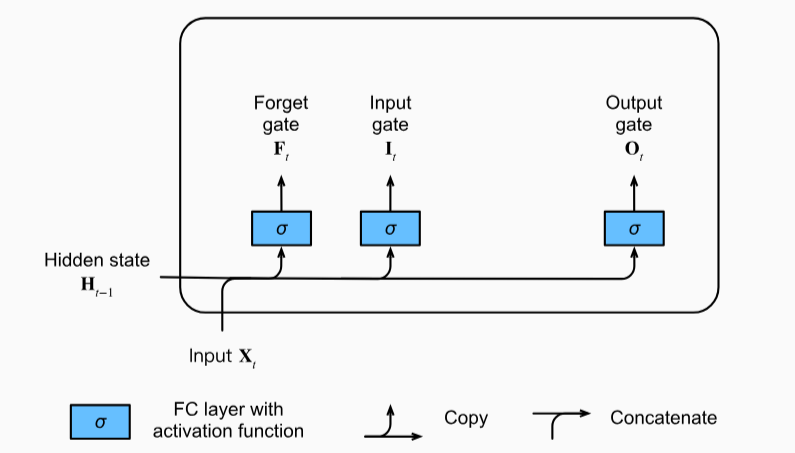
\includegraphics[width=0.7\linewidth]{lstm1}
	\caption{محاسبه گیت ورودی،‌ فراموشی و خروجی در یک سلول LSTM}
	\label{fig:lstm1}
\end{figure}

در مدل‌های شبکه‌های عصبی بازگشتی (RNN)، فرض کنید که تعداد واحدهای پنهان برابر با \( h \)، اندازه دسته برابر با \( n \) و تعداد ورودی‌ها برابر با \( d \) باشد. بنابراین، ورودی به شبکه در زمان گام \( t \) به صورت \( \mathbf{X}_t \in \mathbb{R}^{n \times d} \) و وضعیت پنهان گام زمانی قبلی به صورت \( \mathbf{H}_{t-1} \in \mathbb{R}^{n \times h} \) تعریف می‌شود. به طور مشابه، در هر زمان گام \( t \)، گیت‌ها به شرح زیر تعریف می‌شوند: گیت ورودی \( \mathbf{I}_t \in \mathbb{R}^{n \times h} \)، گیت فراموشی \( \mathbf{F}_t \in \mathbb{R}^{n \times h} \) و گیت خروجی \( \mathbf{O}_t \in \mathbb{R}^{n \times h} \). این گیت‌ها به صورت زیر محاسبه می‌شوند:

\[
\begin{aligned}
	\mathbf{I}_t &= \sigma(\mathbf{X}_t \mathbf{W}_{\textrm{xi}} + \mathbf{H}_{t-1} \mathbf{W}_{\textrm{hi}} + \mathbf{b}_\textrm{i}),\\
	\mathbf{F}_t &= \sigma(\mathbf{X}_t \mathbf{W}_{\textrm{xf}} + \mathbf{H}_{t-1} \mathbf{W}_{\textrm{hf}} + \mathbf{b}_\textrm{f}),\\
	\mathbf{O}_t &= \sigma(\mathbf{X}_t \mathbf{W}_{\textrm{xo}} + \mathbf{H}_{t-1} \mathbf{W}_{\textrm{ho}} + \mathbf{b}_\textrm{o}),
\end{aligned}
\]

که در آن \( \mathbf{W}_{\textrm{xi}}, \mathbf{W}_{\textrm{xf}}, \mathbf{W}_{\textrm{xo}} \in \mathbb{R}^{d \times h} \) و \( \mathbf{W}_{\textrm{hi}}, \mathbf{W}_{\textrm{hf}}, \mathbf{W}_{\textrm{ho}} \in \mathbb{R}^{h \times h} \) پارامترهای وزن هستند و \( \mathbf{b}_\textrm{i}, \mathbf{b}_\textrm{f}, \mathbf{b}_\textrm{o} \in \mathbb{R}^{1 \times h} \) پارامترهای بایاس هستند. در اینجا، از توابع سیگموید استفاده می‌شود تا مقادیر ورودی به بازه \( (0, 1) \) نگاشت شوند.


\subsection{جاری کردن داده های تصویری در LSTM}


شبکه‌های LSTM به‌طور ذاتی برای داده‌های ترتیبی طراحی شده‌اند، درحالی‌که تصاویر داده‌های دو یا سه بعدی \((\mathbf{I} \in \mathbb{R}^{H \times W \times C})\) هستند. بنابراین، برای استفاده از تصاویر در یک معماری ترتیبی مانند \lr{LSTM}، نیاز به تغییر شکل و پیش‌پردازش داده‌های تصویری داریم. در ادامه مراحل و رویکردهای ممکن توضیح داده می‌شوند.

\subsection{تبدیل تصویر به داده‌های ترتیبی}

از آنجایی که LSTM داده‌ها را به صورت دنباله‌ (\lr{Sequence}) پردازش می‌کند، تصویر باید به شکل یک توالی تغییر داده شود. چند روش معمول برای این کار وجود دارد:

\subsubsection{مسطح‌سازی سطرها (\lr{Row-wise Flattening})}

در این روش، هر سطر تصویر به یک گام زمانی (\lr{Time Step}) تبدیل می‌شود. این مسطح‌سازی می‌تواند هر عملی روی فضای پیکسلی $I$ باشد که تبدیل زیر را پیاده‌سازی می‌کند:
\[
\mathbf{I} \in \mathbb{R}^{H \times W \times C} \quad \rightarrow \quad \mathbf{X} \in \mathbb{R}^{H \times (W \cdot C)}
\]
در اینجا:
\begin{itemize}
	\item \(H\): تعداد سطرهای تصویر که به تعداد گام‌های زمانی تبدیل می‌شود.
	\item \(W \cdot C\): تعداد ویژگی‌های هر سطر (عرض تصویر ضربدر تعداد کانال‌ها) که به بردار ویژگی تبدیل می‌شود.
\end{itemize}

\subsubsection{مسطح‌سازی ستون‌ها (\lr{Column-wise Flattening})}

در این روش، هر ستون تصویر به یک گام زمانی تبدیل می‌شود. در نتیجه:
\[
\mathbf{I} \in \mathbb{R}^{H \times W \times C} \quad \rightarrow \quad \mathbf{X} \in \mathbb{R}^{W \times (H \cdot C)}
\]
ایده مشابه حالت سطری است، اما در اینجا ستون‌ها به عنوان گام‌های زمانی در نظر گرفته می‌شوند.

\subsubsection{مسطح‌سازی مبتنی بر پچ‌ها (\lr{Patch-based Flattening})}

برای افزایش انعطاف‌پذیری مدل، می‌توان تصویر را به پچ‌های کوچک تقسیم کرد (شبیه
\cite{dosovitskiyImageWorth16x162021}
). هر پچ به یک گام زمانی تبدیل می‌شود:
\[
\mathbf{I} \in \mathbb{R}^{H \times W \times C} \quad \rightarrow \quad \mathbf{X} \in \mathbb{R}^{T \times (P^2 \cdot C)}
\]
در اینجا:
\begin{itemize}
	\item \(P \times P\): ابعاد هر پچ.
	\item \(T = \frac{H \times W}{P^2}\): تعداد کل پچ‌ها که برابر با طول دنباله \lr{(Sequence Length)} است.
	\item \(P^2 \cdot C\): تعداد ویژگی‌ها در هر گام زمانی.
\end{itemize}

\subsection{پیش‌پردازش ورودی}

پس از مسطح‌سازی، داده‌های تصویری نیازمند پیش‌پردازش‌های زیر هستند:
\begin{itemize}
	\item \textbf{نرمال‌سازی مقادیر پیکسل:} مقادیر تصویر به بازه \([0, 1]\) یا استانداردسازی با میانگین و واریانس تبدیل شوند.
	\item \textbf{استخراج ویژگی با CNN:} برای افزایش دقت، می‌توان پیش از ورود داده به LSTM، ویژگی‌های فضایی تصویر را با شبکه‌های CNN استخراج کرد.
\end{itemize}

\subsection{مدلسازی با LSTM}

پس از آماده‌سازی داده، توالی تولید شده \((\mathbf{X} \in \mathbb{R}^{T \times d})\) مستقیماً به LSTM داده می‌شود. در اینجا \(T\) تعداد گام‌های زمانی و \(d\) ابعاد ویژگی در هر گام است:
$$
\mathbf{H}_t = \textrm{LSTM}(\mathbf{X}_t, \mathbf{H}_{t-1})
$$
که در آن:
\(\mathbf{X}_t \in \mathbb{R}^d\)
بردار ویژگی در گام زمانی $t$ است و
\(\mathbf{H}_t \in \mathbb{R}^h\)
وضعیت پنهان LSTM در گام $t$ است.

\subsection{بازسازی تصویر}

پس از پردازش توالی توسط LSTM، خروجی آن باید به تصویر بازسازی شود. این بازسازی بسته به نوع پیش‌پردازش به یکی از روش‌های زیر انجام می‌شود:
\begin{itemize}
	\item تبدیل مستقیم بردارها به پیکسل‌ها (در حالت مسطح‌سازی سطری یا ستونی).
	\item بازسازی پچ‌ها و ادغام آن‌ها برای تولید تصویر کامل.
\end{itemize}

\subsection{رویکرد هیبریدی CNN-LSTM (پیشنهادشده)}
مدل‌های هیبریدی که از ترکیب شبکه‌های عصبی کانولوشنی (CNN) و حافظه طولانی‌کوتاه‌مدت (LSTM) بهره می‌برند، به عنوان راهکاری قدرتمند برای پردازش داده‌هایی که هم جنبه‌های فضایی و هم جنبه‌های زمانی را شامل می‌شوند، مطرح شده‌اند
\cite{shiConvolutionalLSTMNetwork2015}.
LSTM
 ها به طور ذاتی برای داده‌های ترتیبی طراحی شده‌اند و در درک روابط زمانی عملکرد بالایی دارند؛ اما قدرت لازم برای استخراج روابط مکانی و وابستگی های محلی فضایی در داده‌هایی نظیر تصاویر بزرگ را ندارند. از سوی دیگر، شبکه های کانولوشنی توانایی استخراج این ویژگی‌های مکانی از داده‌های تصویری دارند. بنابراین، ترکیب این دو معماری امکان بهره‌گیری از مزایای هر دو مدل را فراهم می‌کند.

در این رویکرد، ابتدا تصویر ورودی به کمک یک شبکه کانولوشنی به ویژگی‌هایی با سطح بالاتر تبدیل می‌شود. این ویژگی‌ها در قالب یک بردار چندبعدی $\mathbf{F} \in \mathbb{R}^{H' \times W' \times C'}$ بیان می‌شوند که در آن $H'$ و $W'$ ابعاد فضایی فشرده ویژگی‌ها و $C'$ تعداد فیتلر‌ها در آخرین لایه کانولوشنی را نشان می‌دهد. پس از استخراج ویژگی، داده‌ها به یک دنباله $\mathbf{X} \in \mathbb{R}^{T \times d}$ تبدیل می‌شوند، جایی که $T$ طول دنباله و $d$ ابعاد ویژگی‌های استخراج‌شده در هر گام زمانی است. این دنباله سپس به یک LSTM داده می‌شود تا وابستگی‌های زمانی موجود در داده‌ها را مدل‌سازی کند. در نهایت، خروجی این فرآیند می‌تواند برای بازسازی تصویر یا انجام وظایف دیگر از قبیل طبقه‌بندی یا پیش‌بینی استفاده شود. در موارد بازسازی تصویر، یک لایه تمام‌متصل یا یک کدگشای کانولوشنی برای بازسازی دقیق‌تر استفاده می‌شود.

گیت‌های ورودی، فراموشی، و خروجی و همچنین سلول کاندید به صورت زیر تعریف می‌شوند:
\[
\begin{aligned}
	\mathbf{I}_t &= \sigma \left( \mathbf{W}_{\text{xi}} * \mathbf{X}_t + \mathbf{W}_{\text{hi}} * \mathbf{H}_{t-1} + \mathbf{b}_i \right), \\
	\mathbf{F}_t &= \sigma \left( \mathbf{W}_{\text{xf}} * \mathbf{X}_t + \mathbf{W}_{\text{hf}} * \mathbf{H}_{t-1} + \mathbf{b}_f \right), \\
	\mathbf{O}_t &= \sigma \left( \mathbf{W}_{\text{xo}} * \mathbf{X}_t + \mathbf{W}_{\text{ho}} * \mathbf{H}_{t-1} + \mathbf{b}_o \right), \\
	\tilde{\mathbf{C}}_t &= \tanh \left( \mathbf{W}_{\text{xc}} * \mathbf{X}_t + \mathbf{W}_{\text{hc}} * \mathbf{H}_{t-1} + \mathbf{b}_c \right).
\end{aligned}
\]
در اینجا:
\begin{itemize}
	\item \(*\): عملیات کانولوشن است.
	\item \(\mathbf{W}_{\text{xi}}, \mathbf{W}_{\text{hi}}, \dots\): فیلترهای کانولوشن هستند.
	\item \(\mathbf{X}_t \in \mathbb{R}^{H \times W \times C}\): ورودی در گام زمانی \(t\).
	\item \(\mathbf{H}_{t-1}, \mathbf{C}_{t-1} \in \mathbb{R}^{H \times W \times C'}\): وضعیت پنهان و سلول از گام قبلی.
	\item \(\sigma\): تابع سیگموید.
	\item \(\tanh\): تابع تانژانت هایپربولیک.
\end{itemize}

به‌روزرسانی وضعیت سلول و پنهان به صورت زیر انجام می‌شود:
\[
\begin{aligned}
	\mathbf{C}_t &= \mathbf{F}_t \odot \mathbf{C}_{t-1} + \mathbf{I}_t \odot \tilde{\mathbf{C}}_t, \\
	\mathbf{H}_t &= \mathbf{O}_t \odot \tanh(\mathbf{C}_t).
\end{aligned}
\]
در اینجا:
\begin{itemize}
	\item \(\odot\): ضرب عنصر به عنصر (Element-wise).
	\item \(\mathbf{C}_t\): وضعیت سلول فعلی.
	\item \(\mathbf{H}_t\): وضعیت پنهان فعلی.
\end{itemize}

\begin{figure}
	\centering
	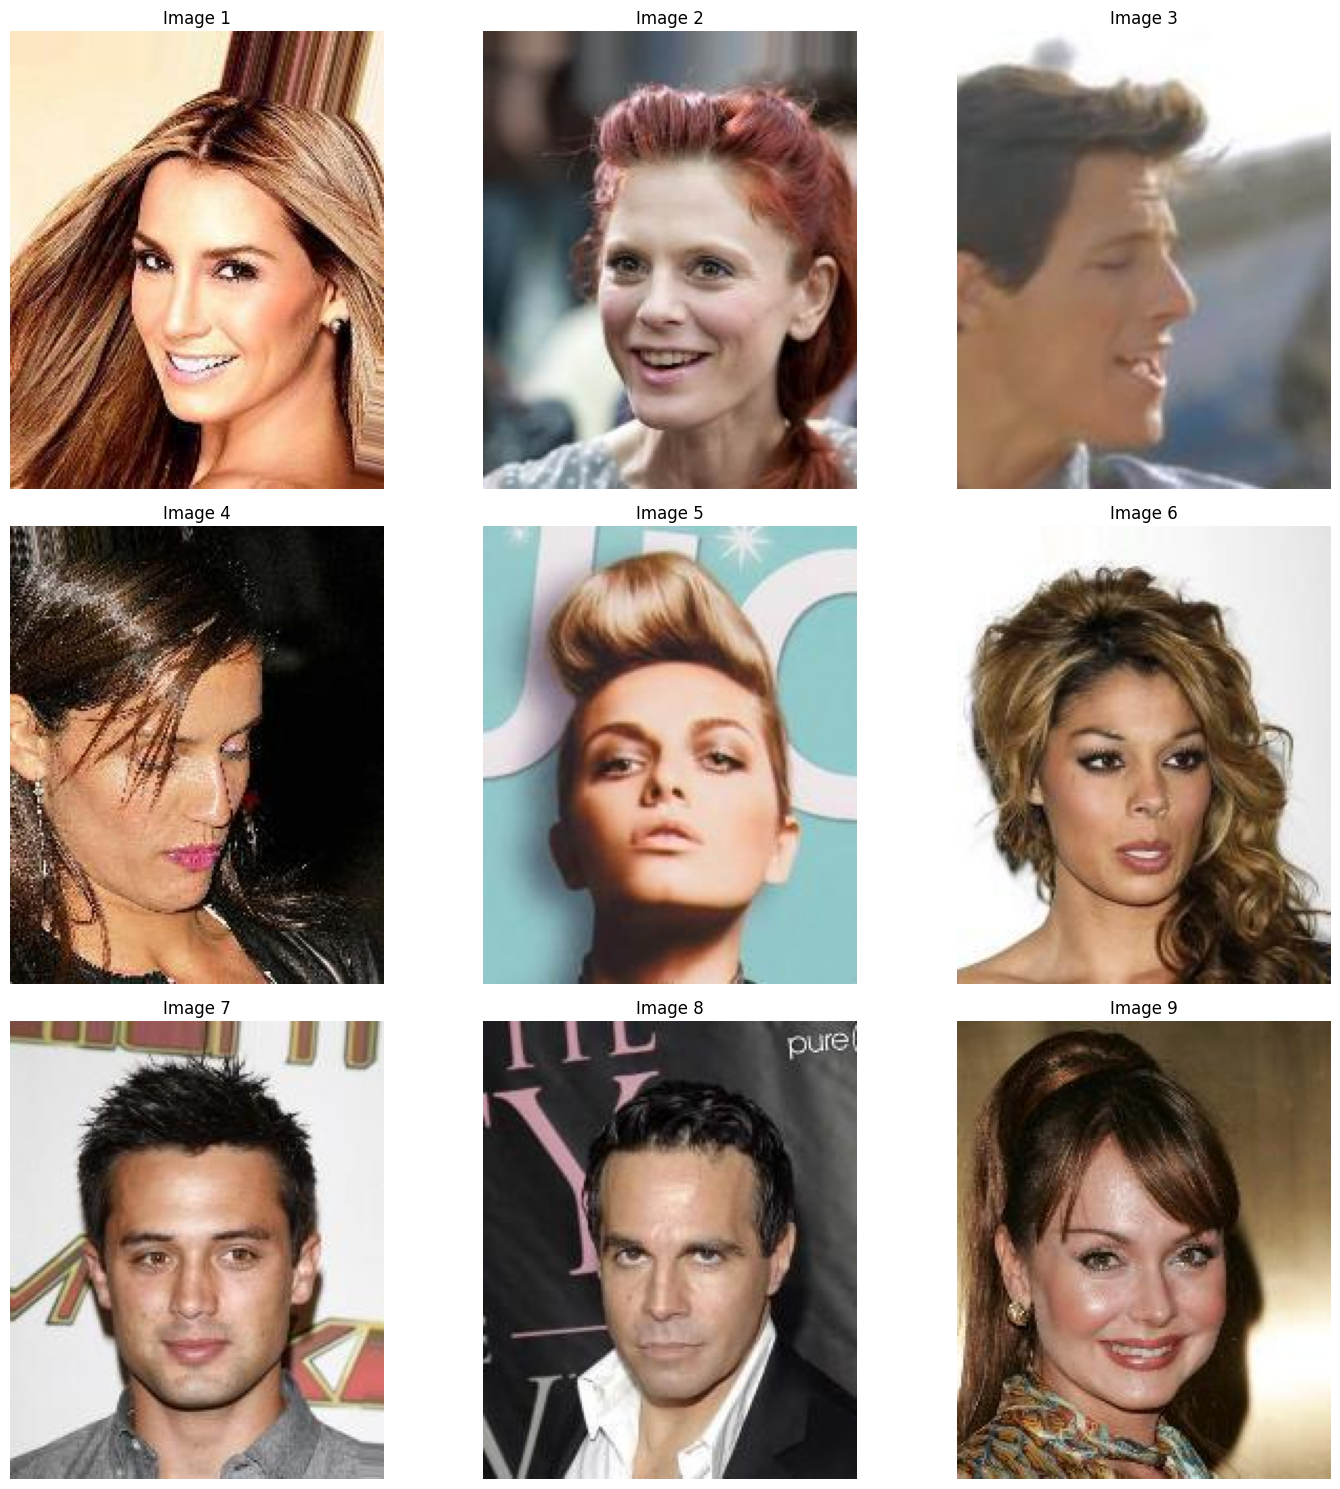
\includegraphics[width=0.7\linewidth]{figs/celebhq2lstm}
	\caption{نمونه ای از مجموعه‌داده مقیاس‌شده و اسپلیت شده استفاده شده تر آموزش مدل های آزمایشی پیشنهادی}
	\label{fig:celebhq2lstm}
\end{figure}


\begin{figure}
	\centering
	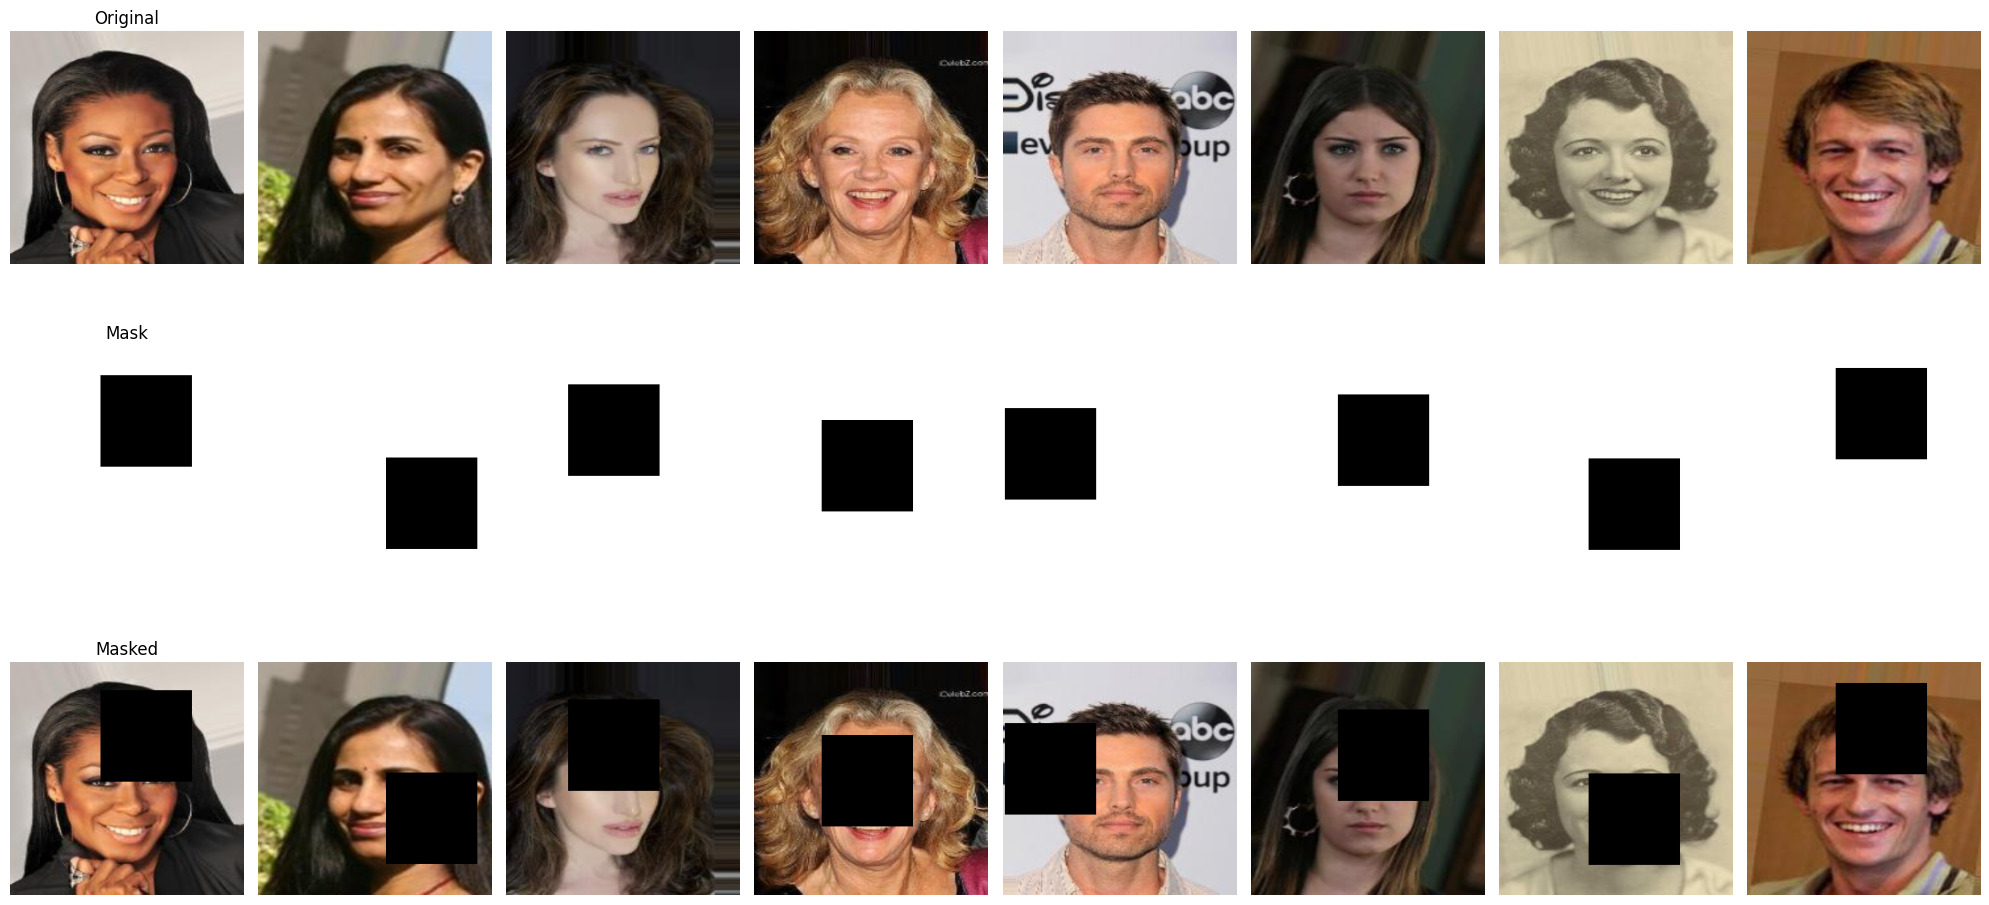
\includegraphics[width=1\linewidth]{figs/lstm1masks}
	\caption{ماسک های مربعی ساخته شده و پیش‌پردازش مجموعه‌داده و آماده سازی برای آموزش}
	\label{fig:lstm1masks}
\end{figure}


\warningToSelfUnfinished
